\chapter{Desenvolvimento}
\label{cap:Desenvolvimento}
Nesse capítulo serão abordadas todas as etapas, tal como as técnicas utilizadas para atingir o objetivo de compor um dicionário de léxicos da língua portuguesa específico para detecção de discursos de ódio promovido pelos usuários chamados de \textit{haters}. Também será apresentada ferramenta implementada que será utilizada como base para as novas funcionalidades e testes com os novos léxicos utilizados .Ao final, também serão apresentados os resultados esperados com o desenvolvimento, estimando a eficiência e os avanços da pesquisa realizada. 

\section{Geração de \textit{corpus} para Detectar \textit{Haters}}
\label{sec:geracaohater}
Como parte fundamental da pesquisa, será criado um dicionário com as palavras mais utilizadas pelos usuários denominados \textit{haters} que pregam discursos de ódio contra indivíduos nas redes sociais. Para a geração do \textit{corpus} desejado serão necessárias algumas etapas de desenvolvimento como pode ser visto na Figura \ref{fig:fluxodesenvolvimento}. A seguir serão explicadas cada uma das etapas a serem realizadas para a obtenção do novo dicionário.

\begin{figure}[!h]
\centering 
\caption{Fluxo de atividades para obtenção de \textit{corpus} desejado}
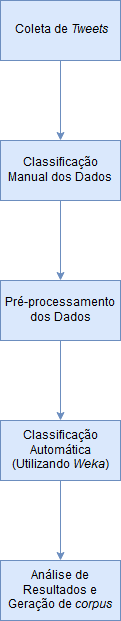
\includegraphics[scale=0.45]{imagens/fluxodesenvolvimento.png}
\legend{Fonte: O Autor}
\label{fig:fluxodesenvolvimento}
\end{figure}

\subsection{Coleta de \textit{Tweets}}
\label{subsec:coletatweets}
A plataforma selecionada para a coleta de dados textuais será o \textit{Twitter}, rede social categorizada como \textit{microblogging} em que os usuários realizam atualizações constantes de conteúdo, sendo esse conteúdo textual, figuras, vídeos, enquetes entre outros. No contexto da rede social, as postagens dos usuários recebem o nome de \textit{tweet} e tem o limite de $280$ caracteres. 

Para realizar a coleta de dados primeiramente é necessário criar uma conta dentro da \textit{Twitter Developer Platform}\footnote{https://developer.twitter.com/} informando alguns tópicos básicos sobre o uso dos dados e a finalidade da ferramenta a ser desenvolvida. Após cadastro, a plataforma disponibilizará os \textit{tokens}\footnote{chaves de autenticação amplamente utilizadas em implementações \textit{OAuth}.Em que não é necessário informar usuário e senha de acesso à ferramenta} que serão necessários para a construção do programa de leitura de \textit{tweets} (Figura \ref{fig:twitterdeveloperplatform}) bem como um painel para controle de acesso aos dados e renovação das \textit{tokens}.

\begin{figure}[!h]
\centering 
\caption{Tela com \textit{tokens} utilizados na \textit{API} do \textit{Twitter}}
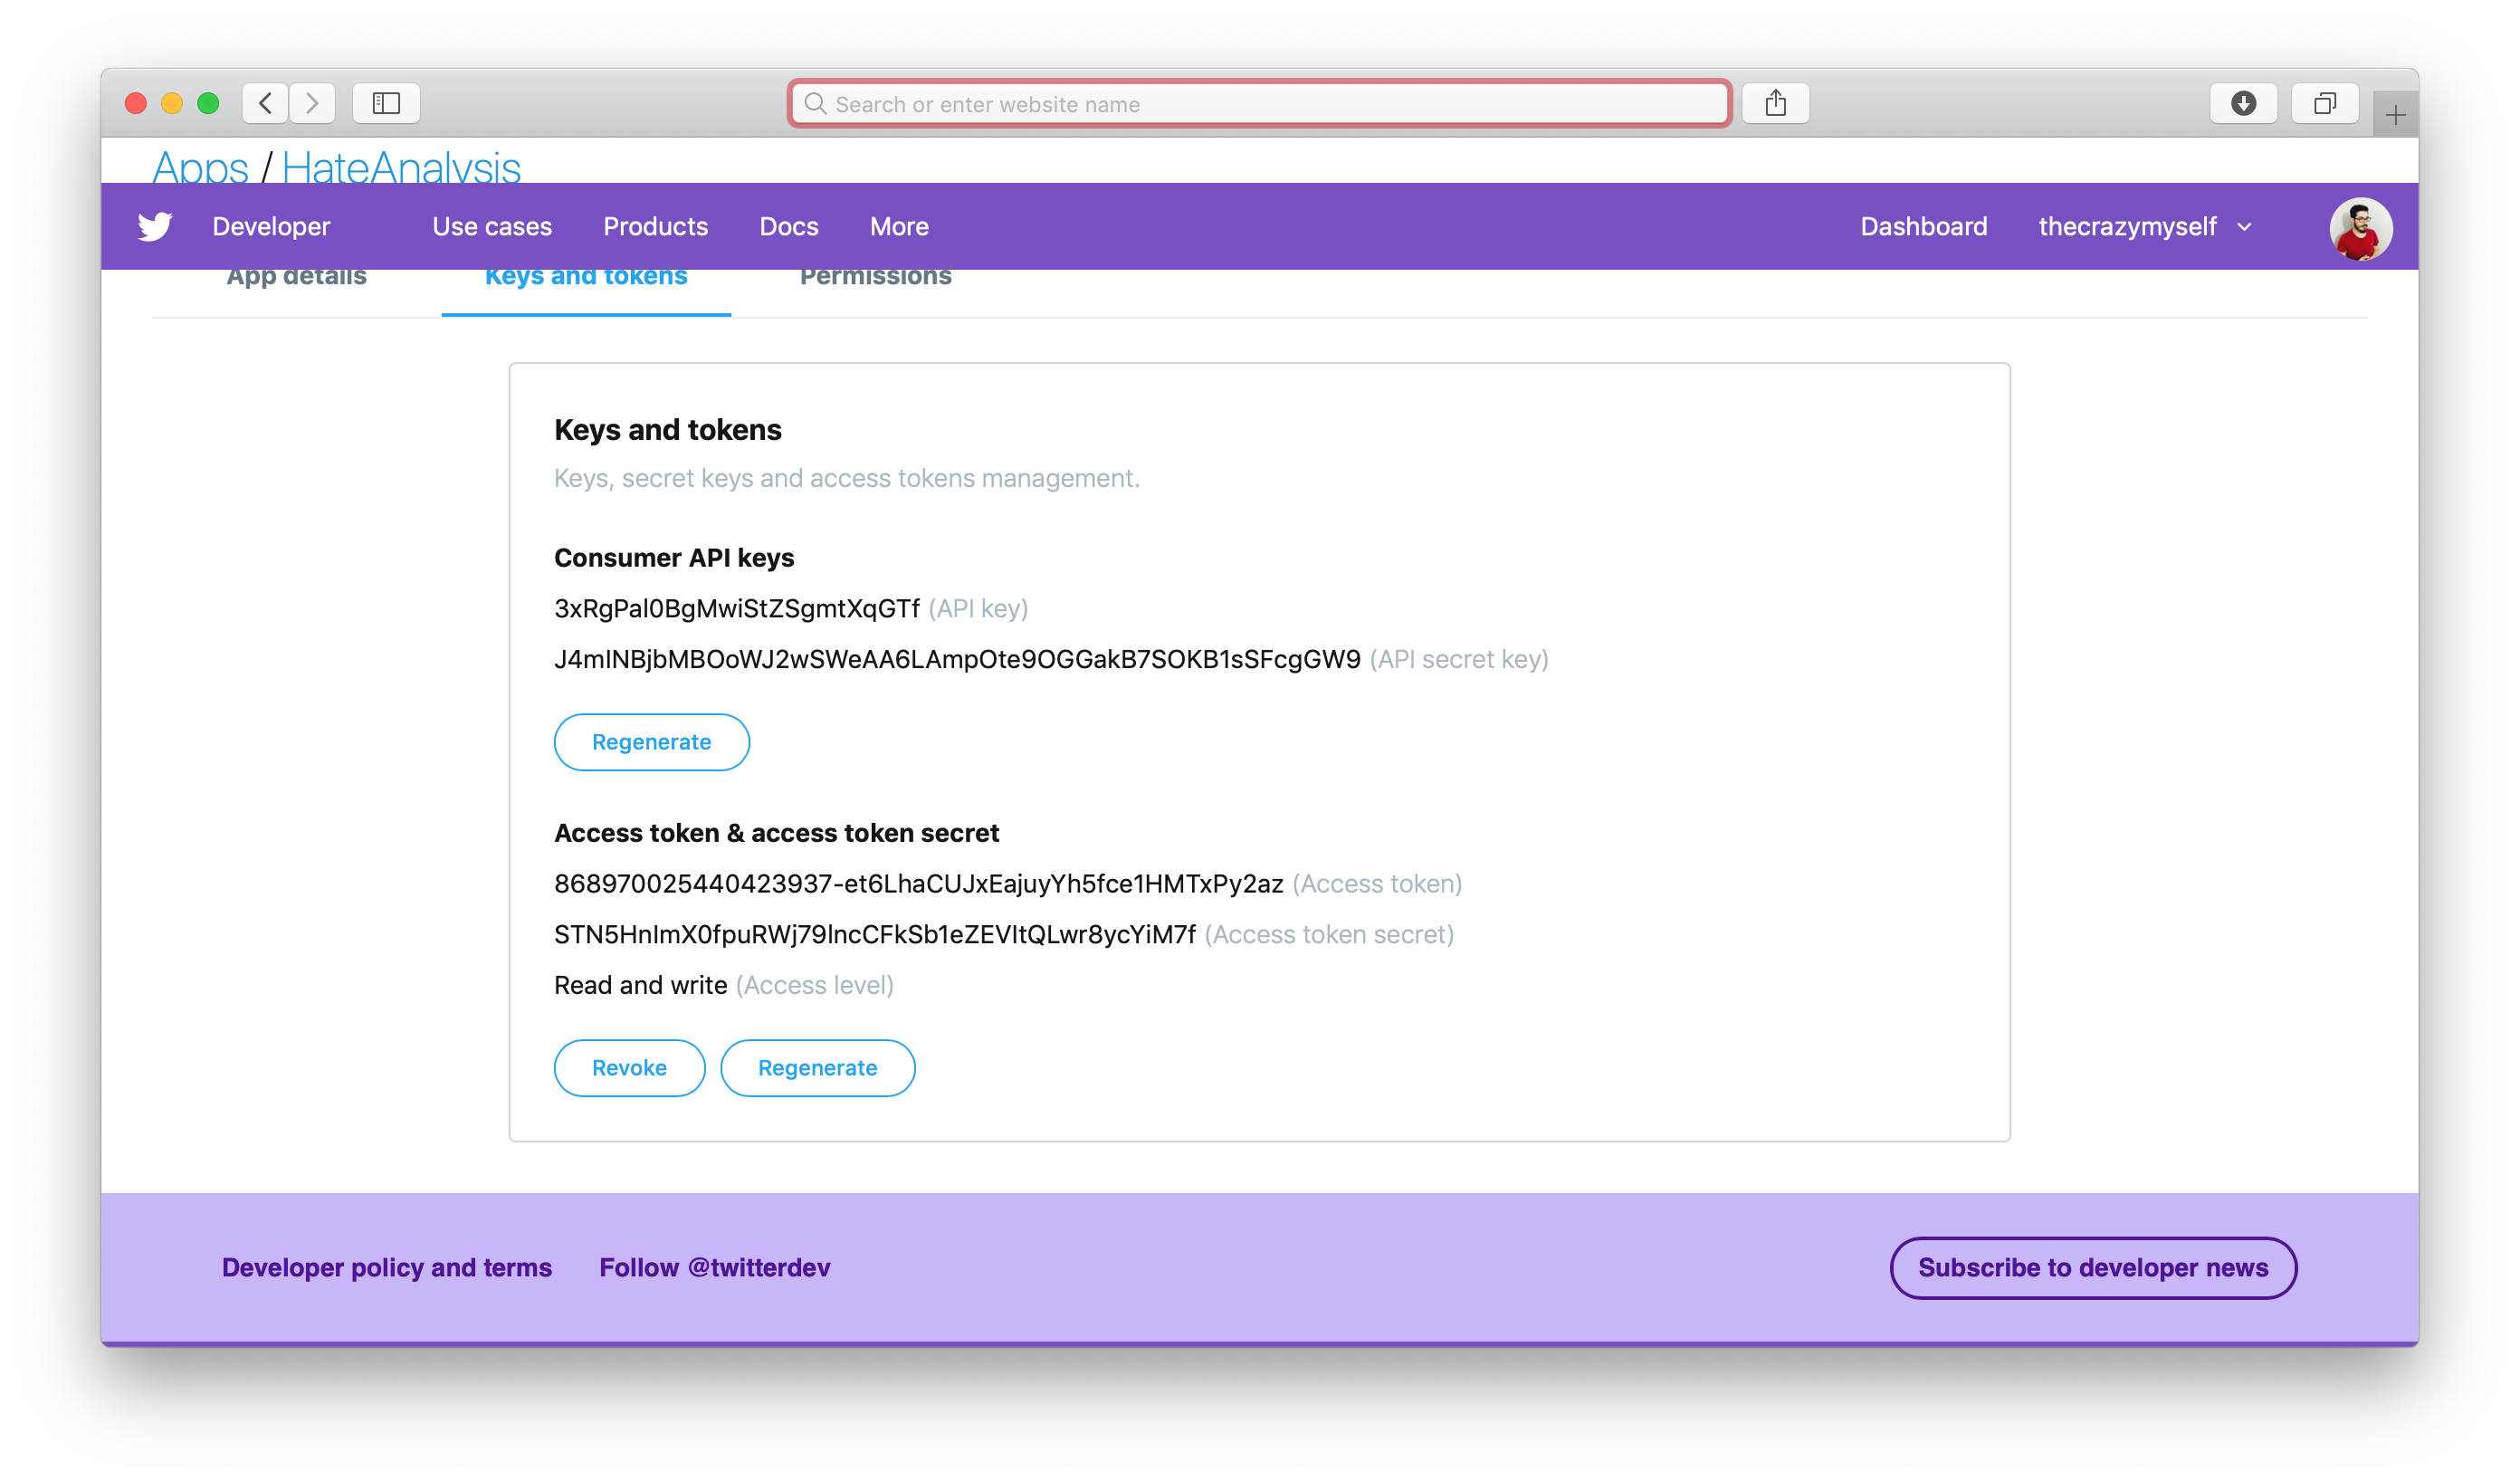
\includegraphics[scale=0.3]{imagens/twitterdeveloperplatform.png}
\legend{Fonte: Twitter Inc.}
\label{fig:twitterdeveloperplatform}
\end{figure}

A linguagem de programação a ser utilizada para a coleta dos dados será a \textit{Java}, linguagem orientada a objetos e multiplataforma mantida pela \textit{Oracle} que é de fácil implementação e bastante utilizada na comunidade \textit{open source} (de código livre) que mantém vários fóruns, \textit{frameworks} e \textit{APIs} constantemente atualizados pela comunidade. A \textit{API} utilizada será a \textit{Twitter4J}\footnote{http://twitter4j.org/en/index.html}, uma biblioteca não-oficial que permite o acesso aos dados do \textit{Twitter} utilizando a linguagem de programação \textit{Java}, a mesma que será utilizada para a coleta de dados, facilitando o aprendizado da ferramenta bem como a manutenção, se necessário. A \textit{Twitter4J} utiliza autenticação \textit{OAuth}, ou seja, fazendo uso dos \textit{tokens} disponibilizados pelo \textit{Twitter Developer Platform} e não necessitando de autenticação com e-mail (ou nome de usuário, e senha) a cada acesso realizado. 

Após a construção do programa de coleta de \textit{tweets}, o próximo passo será encontrar filtros de consulta que irão auxiliar na busca por conteúdos úteis para a geração do \textit{corpus}. O primeiro critério de seleção será a busca por perfis de influenciadores digitais (comumente chamados pela versão inglesa \textit{digital influencers}), que são pessoas que tem grande influência na mídia, tendo vários seguidores e também vários \textit{haters} comentando suas postagens. Nesse primeiro momento os próximos filtros serão manualmente aplicados por um especialista humano que realizará a busca por \textit{tweets} neutros e \textit{tweets} considerados de ódio\footnote{Sendo considerado textos que expressem ideologias onde religião, etnia, deficiências ou gênero são ridicularizados.}. 

A classificação bem como os totais de postagens a serem coletadas pelo especialista podem ser vistos na Tabela \ref{tab:classificacaotweets}.
Após a coleta os dados serão inseridos em arquivos binários e estarão prontos para a próxima etapa prevista para a obtenção do dicionário de léxicos para postagens de \textit{haters} na língua portuguesa.
\begin{table}[h!]
  \begin{center}
    \caption{Classificação dos \textit{tweets} coletados por especialista humano}
    \label{tab:classificacaotweets}
    \begin{tabular}{ll} % <-- Alignments: 1st column left, 2nd middle and 3rd right, with vertical lines in between
    \textbf{Classificação} & \textbf{Quantidade de Tweets}\\
    \hline
    \textit{Tweets} Neutros&500 \textit{Tweets}&
    \textit{Tweets} de Ódio&500 \textit{Tweets}&
    \hline
    Total&1.000 \textit{Tweets}\\
    \end{tabular}
  \end{center}
  \legend{Fonte: O Autor}
\end{table}

\subsection{Classificação Manual dos Dados}
\label{subsec:classmanual}
Nessa etapa, com o auxílio de um especialista humano, os textos apurados na etapa de coleta de \textit{tweets} (Sub-sessão \ref{subsec:coletatweets}) passarão por uma classificação manual como pode ser visto na Figura \ref{fig:classificacaotextos}, afim de gerar uma base de dados para posterior aprendizado de máquina e para comparação estatística de resultados. 
Nessa etapa os textos poderão ser classificados entre duas categorias: \textit{neutro} e \textit{hater}. Onde a primeira categoria compreenderá textos sem nenhum tipo de violência nem extremismo, podendo compreender emoções tanto positivas como negativas. Já a segunda categoria compreenderá textos invasivos, onde a violência verbal seja praticada contra um indivíduo ou um grupo. Dentro desses textos violentos pretende-se também classificar as violências nas subcategorias: racista, religioso, incapacidade e gênero.  

\begin{figure}[!h]
\centering 
\caption{Diagrama de coleta e classificação dos textos}
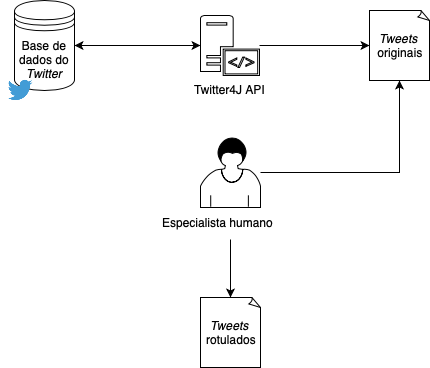
\includegraphics[scale=0.50]{imagens/coletatweets.png}
\legend{Fonte: O Autor}
\label{fig:classificacaotextos}
\end{figure}
\newpage

Com essa etapa pretende-se montar uma base de dados que posteriormente será pré-processada para remoção de ruídos e que irá compor o \textit{dataset} para treinamento dentro do \textit{software Weka}. Por isso, é importante que os textos sigam a seguinte formatação: "classificador, racista (true, false), religioso (true, false), incapacidade (true, false), gênero (false),'texto coletado'" como forma de padronização de dados a serem classificados de forma automática como é exemplificado na Figura \ref{fig:arqanalise} onde pode ser verificado um primeiro texto onde um discurso de ódio foi detectado e sub categorizado como ódio a um gênero e já no segundo texto nada foi percebido e portanto o mesmo foi classificado como neutro.

\begin{figure}[!h]
\centering 
\caption{Exemplo de classificação manual }
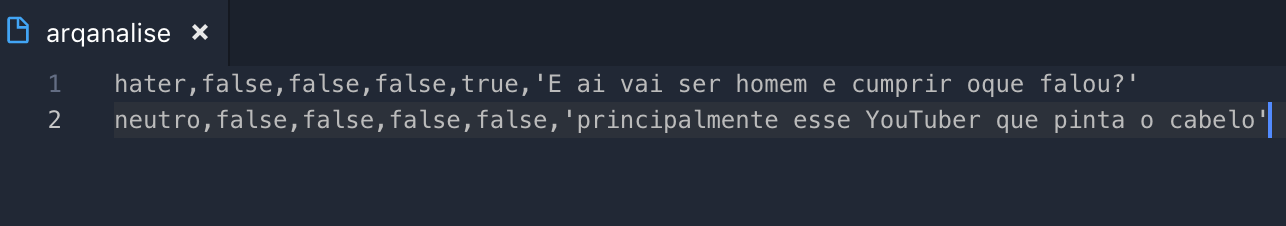
\includegraphics[scale=0.60]{imagens/arqanalise.png}
\legend{Fonte: O Autor}
\label{fig:arqanalise}
\end{figure}

\subsection{Pré-processamento dos \textit{Tweets}}
Assim como visto na Sub-sessão \ref{subsec:preproc}, a etapa de pré-processamento é necessária para a remoção de informações desnecessárias, realizando uma padronização das informações contidas nos textos coletados realizando uma otimização considerável no conteúdo a ser avaliado no processo de classificação automática. 

Para a composição do \textit{dataset} serão realizadas as técnicas de: remoção de conteúdo numérico, remoção de \textit{URL}, remoção de conteúdo numérico, substituição de pontuações repetidas, todas as palavras serão transformadas para letras maiúsculas, remoção de palavras \textit{stopwords} e substituição de palavras alongadas. 

Ao realizar as técnicas citadas anteriormente, será gerado um \textit{dataset} otimizado. O mesmo será utilizado na etapa de classificação e treinamento de máquina para a geração do \textit{corpus} objetivo do trabalho. Posteriormente a mesma rotina de pré-classificação será incorporada em ferramenta desenvolvida citada na Sessão \ref{sec:revisaoferramenta}.

\subsection{Classificação Automática Utilizando o \textit{Weka} e Geração de \textit{corpus}}

Tendo realizado as etapas anteriores de coleta de \textit{tweets}, de classificação manual e de pré-processamento, o próximo passo será a aplicação de algoritmos de \textit{machine learning} para a classificação automática dos dados apurados nas etapas anteriores. A ferramenta utilizada nessa etapa será o \textit{software} chamado \textit{Weka} \footnote{https://www.cs.waikato.ac.nz/ml/weka/}(Figura \ref{fig:telaincialweka}) que é uma coleção de algoritmos de \textit{machine learning} utilizados para tarefas de mineração de dados, contendo ferramentas para preparação, classificação, clusterização, entre outros.  Além de ter ferramentas de visualização de resultados. O \textit{Weka} é um \textit{software} \textit{open source} sob a \textit{GNU General Public License}\footnote{https://www.gnu.org/licenses/licenses.html\#GPL} \cite{weka_2018}.

\begin{figure}[!h]
\centering 
\caption{Tela inicial da ferramenta \textit{Weka}}
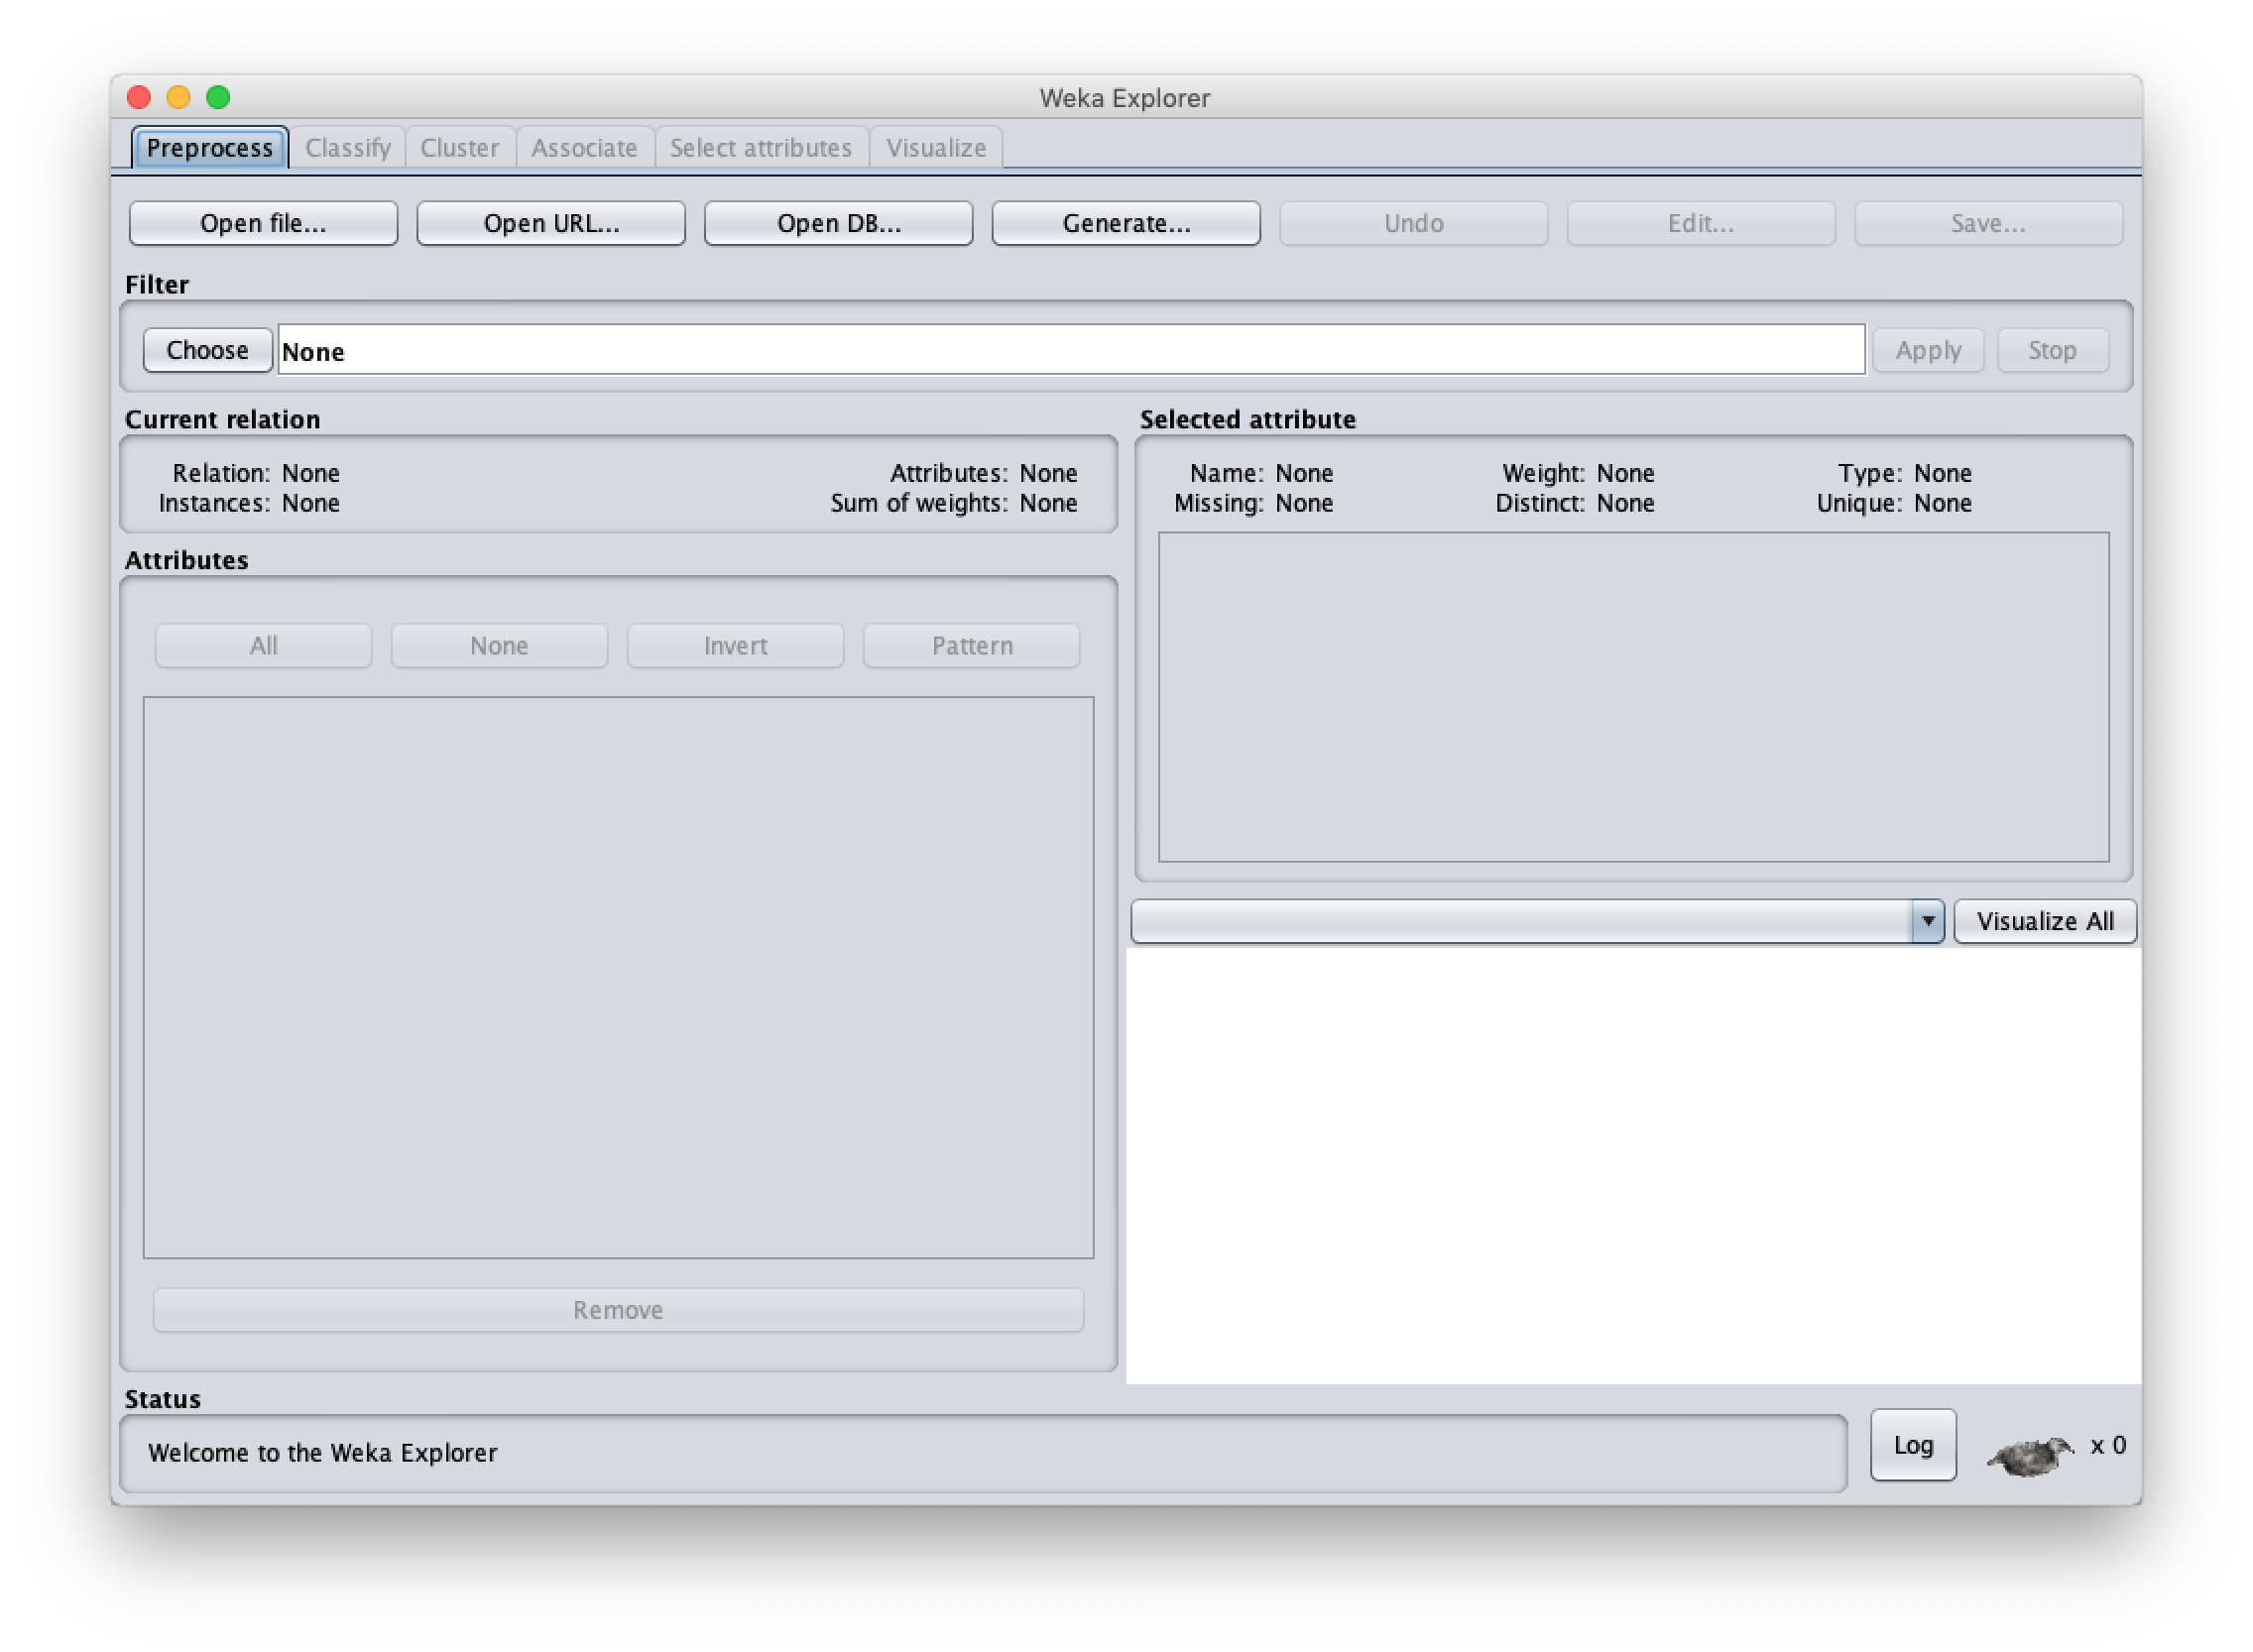
\includegraphics[scale=0.33]{imagens/wekatelainicial.png}
\legend{Fonte: O Autor}
\label{fig:telaincialweka}
\end{figure}

Essa etapa pretende executar três algoritmos de classificação automática de textos para, a partir de seus resultados, gerar o \textit{corpus} com os léxicos mais utilizados nos discursos de ódio. Um esquema com os passos principais pode ser visto na Figura \ref{fig:wekaclassificacao}. Os três algoritmos a serem utilizados nessa etapa são: \textit{Naive Bayes} (NB), \textit{Bayse net} (BN) e \textit{Support Vector Machine} (SVM) \cite{Muralidharan2012,N18-1095}. 

\begin{figure}[!h]
\centering 
\caption{Diagrama da etapa de classificação com o \textit{software} \textit{Weka}}
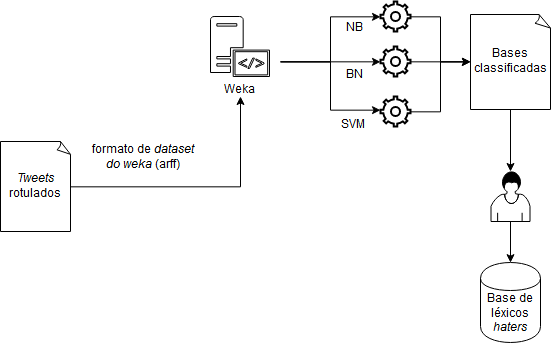
\includegraphics[scale=0.50]{imagens/wekaclassificacao.png}
\legend{Fonte: O Autor}
\label{fig:wekaclassificacao}
\end{figure}

\section{Revisão de Ferramenta Implementada}
\label{sec:revisaoferramenta}
Com o crescimento das pesquisas no campo da mineração de texto e com as variadas aplicações encontradas para a análise de sentimentos, cada vez mais ferramentas são desenvolvidas com os mais variados propósitos de pesquisa e também para aplicações comerciais. A ferramenta base para o trabalho aqui desenvolvido é resultado de uma pesquisa realizada por \citeonline{tccfilipe} que resultou em um \textit{software} \textit{web crawler}\footnote{ \textit{Softwares} que criam conexão com determinado \textit{site} e extraem informações desejadas por meio de APIs geralmente disponibilizadas pelo meio eletrônico.} que realiza a análise de sentimentos em uma interface relativamente simples para usuários que não têm experiência em programação.

É possível verificar na Figura \ref{fig:fluxotccfilipe} o fluxo de funcionalidades da ferramenta implementada onde, inicialmente, o usuário entra com uma URL de busca e a quantidade de postagens a ser analisada (Figura \ref{fig:menutccfilipe}) e após ocorre a classificação e por fim ocorre a apresentação das informações em forma de nuvem de palavras (Figura \ref{fig:nuvemtccfilipe}), gráficos (Figura \ref{fig:graficotccfilipe}), e ainda, em relatórios gerados em PDF (Figura \ref{fig:exportadotccfilipe}). A coleta de dados ocorreu com a API apresentada na sub-sessão \ref{subsec:coletadados} chamada \textit{Facebook Graph API}, a partir dela o \textit{software} faz buscas na rede social \textit{Facebook} e coleta postagens conforme parametrizado.

\newpage

\begin{figure}[!h]
\centering 
\caption{Fluxograma de funcionalidades do \textit{software} revisado}
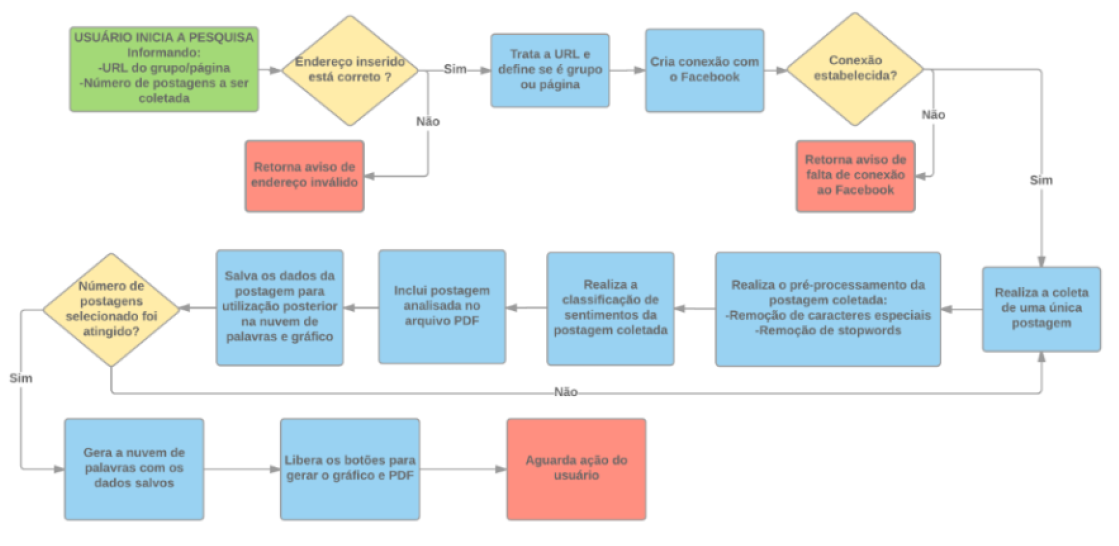
\includegraphics[scale=0.40]{imagens/fluxofilipe.png}
\legend{Fonte: \citeauthor{tccfilipe}}
\label{fig:fluxotccfilipe}
\end{figure}

\begin{figure}[!h]
\centering 
\caption{Menu de busca do \textit{software} revisado}
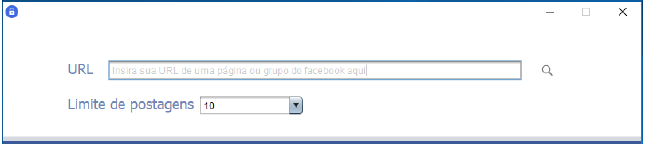
\includegraphics[scale=0.5]{imagens/menudebuscafilipe.png}
\legend{Fonte: \citeauthor{tccfilipe}}
\label{fig:menutccfilipe}
\end{figure}

\begin{figure}[!h]
\centering 
\caption{Nuvem de palavras do \textit{software} revisado}
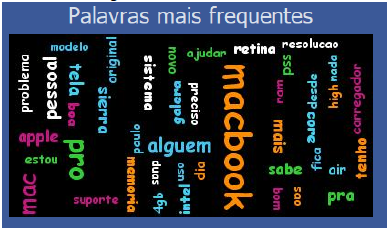
\includegraphics[scale=0.62]{imagens/nuvemdepalavras.png}
\legend{Fonte: \citeauthor{tccfilipe}}
\label{fig:nuvemtccfilipe}
\end{figure}

\begin{figure}[!h]
\centering 
\caption{Gráfico de sentimentos do \textit{software} revisado}
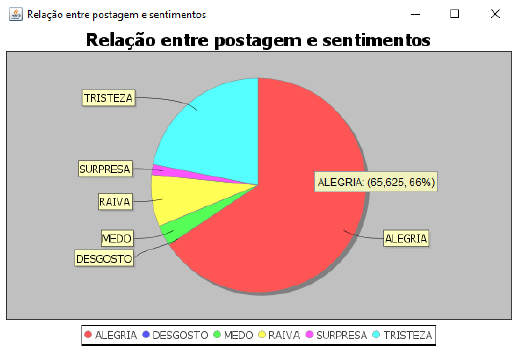
\includegraphics[scale=0.8]{imagens/graficodesentimentosfilipe.png}
\legend{Fonte: \citeauthor{tccfilipe}}
\label{fig:graficotccfilipe}
\end{figure}

\begin{figure}[!h]
\centering 
\caption{Resultado exportado do \textit{software} revisado}
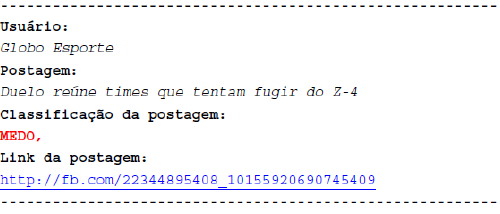
\includegraphics[scale=0.60]{imagens/exportadofilipe.png}
\legend{Fonte: \citeauthor{tccfilipe}}
\label{fig:exportadotccfilipe}
\end{figure}

\newpage
Para atingir o propósito de sua pesquisa, \citeonline{tccfilipe} realizou o estudo de léxicos de emoções contidos na base de dados chamada \textit{WordNet}\footnote{https://wordnet.princeton.edu} categorizados em seis grupos distintos que foram: alegria, desgosto, medo, raiva, surpresa e tristeza. Na Tabela \ref{tab:categoriaemo} estão alguns exemplos de palavras separadas pelas respectivas categorias de emoção selecionado pelo autor. Além da análise de sentimentos também foi implementada busca por palavras frequentemente encontradas em ataques de \textit{phishing},  e também palavras de linguagem imprópria, visto que as redes sociais não mantém um filtro de conteúdo levando em consideração a idade do usuário.

\begin{table}[h!]
  \begin{center}
    \caption{Categorias de emoções}
    \label{tab:categoriaemo}
    \begin{tabular}{ll} % <-- Alignments: 1st column left, 2nd middle and 3rd right, with vertical lines in between
      \textbf{Categoria} & \textbf{Palavras}\\
      \hline
      Alegria&animação, ânimo, comédia\\
      Desgosto&maldoso, chatear, abominável\\
      Medo&desespero, escuridão, friamente\\
      Raiva&assassinar, bravejar, detestar\\
      Surpresa&chocante, espanto, impressionado\\
      Tristeza&cabisbaixo, chorão, culpa\\
      \hline
    \end{tabular}
  \end{center}
  \legend{Fonte: \citeauthor{tccfilipe}}
\end{table}
Após definir os grupos de coleta, os dados de coleta para a análise de sentimentos e realizar a classificação dos dados utilizando método de classificação baseado em léxicos, o autor realizou a análise dos resultados para constatar o quão precisa foi a classificação realizada pela ferramenta. \citeonline{tccfilipe} coletou amostras de diferentes tamanhos em todos os grupos analisados totalizando 50 (cinquenta), 100 (cem) e 500 (quinhentos) postagens para, após, serem também analisadas manualmente e assim comparar os resultados. Dentre os grupos estudados estão a página do \textit{Outback Brasil} e o grupo da Previdência Social, alguns ajustes de léxicos foram necessários para que as classificações ocorressem com maior assertividade nos casos de alegria e tristeza. No final foi realizada a comparação entre as classificações e exatificadas as suas respectivas taxas de acerto, a Tabela \ref{tab:taxaacerto} apresenta os resultados obtidos, com eles foi possível verificar que quatro dos sentimentos tiveram taxa de acerto superiores a oitenta por cento. Com o cálculo do desvio padrão foi possível constatar que nos sentimentos com menor classificação refletiam uma grande dispersão em torno da media populacional, resultado de expressões ambíguas e de duplo sentido.

\begin{table}[h!]
  \begin{center}
    \caption{Taxa média de acerto na classificação de postagens analisadas}
    \label{tab:taxaacerto}
    \begin{tabular}{lllllll} % <-- Alignments: 1st column left, 2nd middle and 3rd right, with vertical lines in between
      \textbf{Classificação} & \textbf{Alegria} & \textbf{Medo} & \textbf{Tristeza} & \textbf{Desgosto} & \textbf{Raiva} & \textbf{Surpresa}\\
      \hline
      Taxa de Acerto&52,82\%&90,77\%&81,55\%&88,89\%&91,01\%&75,83\%\\
      Desvio Padrão($\sigma$)&16,06&2,62&5,20&4,61&4,23&9,97\\
      \hline
    \end{tabular}
  \end{center}
  \legend{Fonte: \citeauthor{tccfilipe}}
\end{table}

Ao final dos estudos foi concluído que a ferramenta desenvolvida trouxe resultados satisfatórios tanto pelos resultados obtidos como pela facilidade que a ferramenta desenvolvida trás para os usuários comuns. Ainda, foram apontadas melhorias para os estudos futuros entre elas o desenvolvimento de uma plataforma \textit{web}, aprimoramento nos testes de resultados da análise de sentimentos e também novas abordagens na etapa de classificação dos dados. 
% falar aqui sobre os resultados encontrados pelo filipe

\section{Integração com \textit{Software} Existente}
\label{sec:integracaosoftware}
Após a composição do \textit{corpus} com as palavras mais utilizadas em discursos de ódio, a nova etapa será agregar essa nova lista ao \textit{software} mencionado na Sessão \ref{sec:revisaoferramenta} para que o mesmo seja capaz de, além de identificar as seis categorias de emoção (alegria, desgosto, medo, raiva, surpresa e tristeza), identificar palavras impróprias e de possíveis ataques de \textit{phishing}, também identifique comentários de ódio comumente praticados pelos \textit{haters}.
Também será necessária a integração com o \textit{Twitter} por meio da API \textit{Twitter4J} já que o \textit{software} está integrado atualmente com o \textit{Facebook} (Figura \ref{fig:implementacao}). 

\begin{figure}[!h]
\centering 
\caption{Diagrama de integração \textit{software} existente}
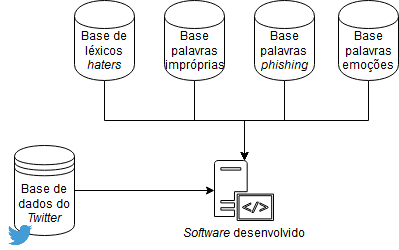
\includegraphics[scale=0.6]{imagens/implementacao.png}
\legend{Fonte: O Autor}
\label{fig:implementacao}
\end{figure}
Após a integração mencionada o trabalho atingirá seu objetivo geral e testes serão realizados para verificação de assertividade nas detecções de discursos de ódio dentre as subcategorias mencionadas na Sub-sessão \ref{subsec:classmanual}.

\section{Resultados Esperados}
Durante o desenvolvimento do trabalho, serão realizadas etapas que compõem a Análise de Sentimentos onde as mesmas serão aplicadas a um problema prático de detecção de discursos de ódio extraindo essas informações a partir de textos extraídos da rede social \textit{Twitter}.

Após a geração de base de dados rotulada manualmente por especialista humano a partir de amostras extraídas da rede mencionada, serão aplicados algoritmos supervisionados de classificação automática de textos e o de melhor desempenho irá auxiliar na composição de \textit{corpus} com as palavras mais frequentes em discursos de ódio. Com o \textit{software} integrado com novo \textit{corpus} pretende-se realizar testes com base aleatória de dados para realizar comparações e verificar a efetividade na detecção de discursos de ódio bem como a subcategoria que o texto compõe (discurso de raça, religião, gênero, incapacidade).